\subsection{Collaboration Mechanisms in LLM-MAS}

Collaboration mechanisms in LLM-based multi-agent systems (LLM-MAS) define how agents decompose tasks, exchange intermediate results, use tools, refine hypotheses, and compose a final solution.
Contemporary surveys examine these mechanisms along several dimensions, including the number and types of agents, communication structure, coordination protocol, role specialization, and solution aggregation methods \cite{tran2025collaboration}.
Contemporary surveys typically examine these mechanisms along several dimensions: the number and types of agents, communication structure, coordination protocol, role specialization, and solution aggregation methods \cite{tran2025collaboration}.
\highlight{Recent work} further highlights the transition from fixed collaboration patterns toward more adaptive coordination and learning strategies, in which agent interactions can be adjusted according to the task and the evolving state of the problem \cite{yarmohammadtoosky2026llm}.
We categorize collaboration mechanisms in LLM-MAS into several major groups as shown in Figure \ref{figure:collaboration_mechanisms}.

\begin{figure}
    \centering
    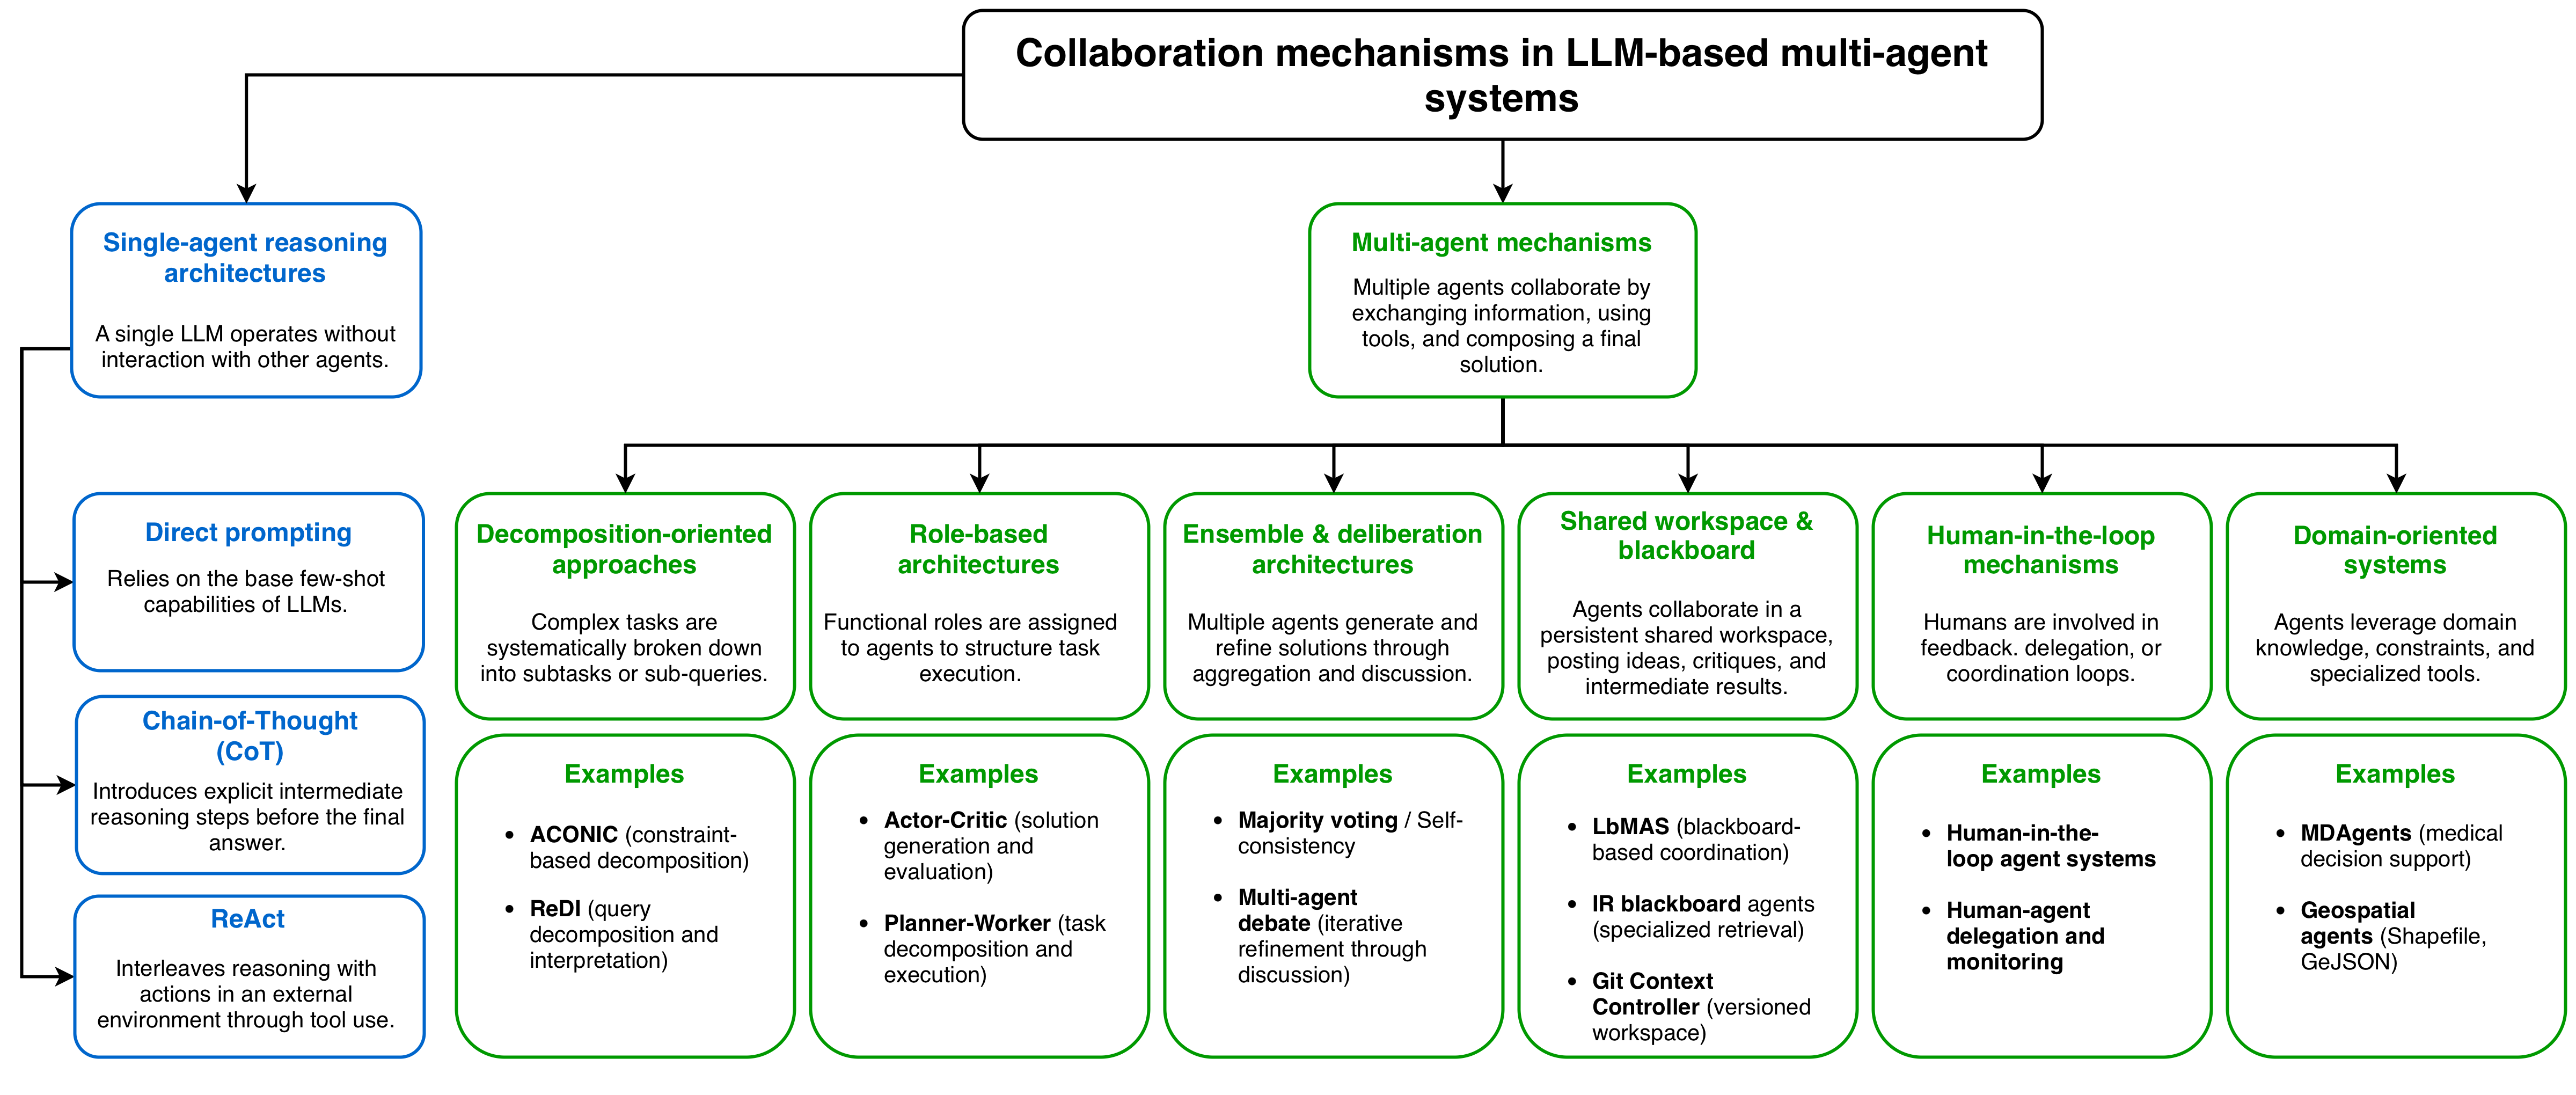
\includegraphics[width=1.0\linewidth]{Sections//2_related_work//Figures/Collaboration mechanisms.png}
    \caption{Collaboration mechanisms in LLM-based multi-agent systems.}
    \label{figure:collaboration_mechanisms}
\end{figure}

\subsubsection{Single-Agent Reasoning Architectures}

The simplest reasoning setting involves a single LLM operating without interaction with other agents.
This group includes direct prompting approaches, which rely on the base few-shot capabilities of large language models \cite{brown2020language}.
A second line of methods extends single-model reasoning through structured intermediate computation.
Chain-of-Thought prompting introduces explicit intermediate reasoning steps before producing a final answer \cite{wei2022chain}, while ReAct interleaves reasoning with actions in an external environment through tool use \cite{yao2023react}.
These approaches cannot be considered multi-agent collaboration mechanisms, but they serve as lower baselines before introducing inter-agent communication.

\subsubsection{Role-Based Architectures}

The second group introduces explicit functional role separation between agents.
In actor–critic approach, one agent produces an initial solution, while another evaluates it, identifies errors, incompleteness, or weaknesses, and provides feedback for refinement.
This logic is related to self-refinement approaches, where a model iteratively improves its own response based on feedback \cite{madaan2023selfrefine}, as well as to contemporary actor–critic frameworks aimed at improving the reliability of LLM agents in multi-step scenarios \cite{jiang2026asymmetric}.
A related pattern is the planner–worker architecture: the planner decomposes the task and manages the execution process, while worker agents solve specialized subtasks.
This approach is often used in domain-oriented systems, including geospatial agents for processing Shapefile and GeoJSON data \cite{lin2025shapefilegpt,luo2026geojson}.
Such architectures are effective when a task can be represented as a sequence of explicit operations, but their communication structure is typically predefined and centralized.

\subsubsection{Ensemble and Deliberation Architectures}

The third group includes ensemble-style and deliberation-based coordination protocols.
Majority voting and self-consistency aggregate several independently generated solutions, reducing the dependence of the result on a single stochastic generation trajectory \cite{wang2023selfconsistency}.
Multi-agent debate extends this idea: multiple agents first independently generate answers, then observe the answers of other agents and refine their own solutions over several rounds \cite{du2023improving}.
However, contemporary research shows that a significant portion of the improvements attributed to debate approaches may be explained not by the debate itself but by the ensemble effect of voting \cite{choi2025debate}. 

\subsubsection{Shared Workspace and Blackboard Systems}

A more flexible group of mechanisms is inspired by collaborative problem-solving systems used in real-world settings involving open-ended and ill-structured tasks.
Blackboard architectures assume a shared workspace in which specialized agents can post partial solutions, facts, hypotheses, criticisms, and intermediate conclusions.
The classic blackboard model was developed for complex, ill-structured problems requiring the integration of heterogeneous sources of expertise \cite{nii1986blackboard}.
In LLM-MAS, this idea is adapted by coordinating agents not only through fixed rounds of discussion but also through persistent collective memory.
LbMAS follows this direction: agents are selected based on the current state of the blackboard, and the process continues until a consensus solution is reached \cite{han2025blackboard}.
Similar blackboard-based systems have also been proposed for information retrieval tasks, where agents autonomously respond to queries in a shared workspace according to their specialization \cite{salemi2025blackboard}.
Another related direction is context management via a version-controlled workspace: the Git Context Controller treats agent memory as structured context with commit, branch, merge, and context retrieval operations, making long agentic workflows more manageable and reproducible \cite{wu2025gitcontext}.
\highlight{Recent surveys} of LLM-MAS increasingly emphasize persistent shared state, failure attribution, and self-evolution as important components of reliable agent collaboration \cite{qi2026beyond}.
This perspective further motivates shared-workspace architectures for tasks in which intermediate evidence and errors must remain accessible across multiple stages of open-ended problem solving.

\subsubsection{Decomposition-Oriented Approaches}

ACONIC proposes systematic decomposition of complex LLM tasks by formalizing them as constraint satisfaction problems.
The framework uses formal complexity measures to determine suitable decomposition structures \cite{zhou2025aconic}.
ReDI applies decomposition and semantic interpretation to complex search queries: the original user query is broken down into sub-queries, each sub-query is augmented with an interpretation, and then the search results are aggregated \cite{zhong2025redi}.
Although such works are not always multi-agent systems in the strict sense, they provide useful principles of decomposition, interpretation, and aggregation that can be embedded into planner-based and blackboard-based LLM-MAS.

\subsubsection{Human-in-the-Loop and Domain-Oriented Systems}

Domain-oriented architectures take into account that solution quality depends not only on the model's general reasoning ability but also on expert knowledge, domain constraints, and correct interpretation of context.
For example, MDAgents dynamically selects an individual or group interaction structure depending on the complexity of a medical task, simulating real clinical decision-making processes \cite{kim2024mdagents}.
Human-agent systems add another level of control by incorporating a human into delegation, monitoring, feedback, or coordination loops \cite{zou2025humanagent}.
This is especially important for ill-structured decision-support tasks, where the result must be not only formally correct but also interpretable, contextually justified, and aligned with stakeholder constraints.

\subsubsection{Summary}
Overall, existing collaboration mechanisms in LLM-MAS have been developed primarily for question answering, reasoning, information retrieval, coding, and domain benchmark tasks, where an objectively correct or externally verifiable answer is assumed.
For ill-structured applied tasks, including urban planning decision support, the most promising direction is a combination of tool-augmented reasoning, shared workspace mechanisms, explicit decomposition, and role specialization.
Among these, blackboard- and context-management-based mechanisms are particularly relevant, as they support incremental construction of solutions and coordination of heterogeneous agents without requiring a rigid interaction protocol.
Human-in-the-loop integration is an important and promising direction for such systems, however, it remains outside the scope of this work and is left for future investigation.